%%%%%%%%%%%%%%%%%%%% Documentación del código %%%%%%%%%%%%%%%%%%%%


\section{Documentación del código fuente}

La documentación obtenida mediante el programa Doxygen, está \href{DOC_DOXYGEN/index.html}{Doxygen}.
Aquí se puede encontrar las definiciones de las estructuras, al igual que el código fuente de cada módulo, junto a su cabecera .h.

%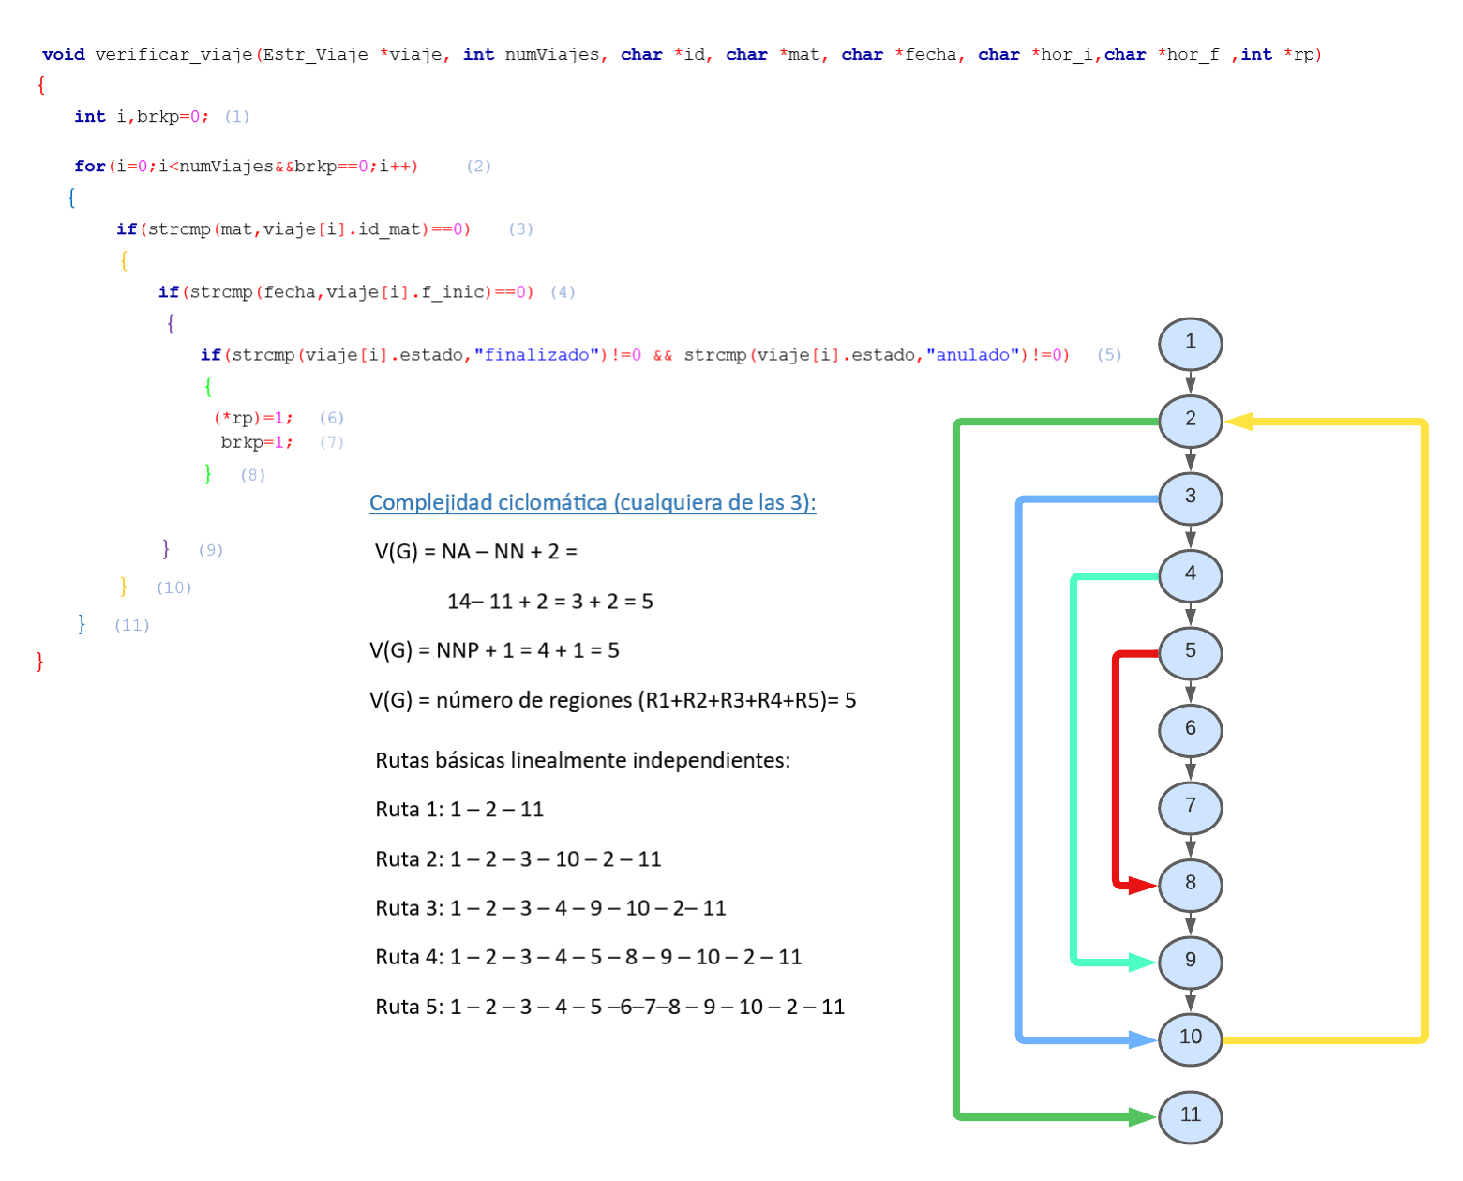
\includepdf[pages={1}]{fotos/123.pdf}

\subsection{Código de los módulos}

En esta parte, se mostrará el código fuente de todos los módulos del proyecto. Se ha puesto al final, para que no moleste a la hora de ver el resto del documento pdf.
\label{fig:CodigoModulos}

\subsubsection{Acceso}

Para ver la descripción del módulo puede ir a \ref{fig:Acceso}.

\label{fig:AccesoCod}
\lstinputlisting[language=C, breaklines=true]{CODIGO_sin_caracteres_especiales/acceso.c}

\subsubsection{Actualizar}

Para ver la descripción del módulo puede ir a \ref{fig:Actualizar}.

\label{fig:ActualizarCod}
\lstinputlisting[language=C, breaklines=true]{CODIGO_sin_caracteres_especiales/actualizar.c}

\subsubsection{Buscar}

Para ver la descripción del módulo puede ir a \ref{fig:Buscar}.

\label{fig:BuscarCod}
\lstinputlisting[language=C, breaklines=true]{CODIGO_sin_caracteres_especiales/buscar.c}

\subsubsection{Colores}

Para ver la descripción del módulo puede ir a \ref{fig:Colores}.

\label{fig:ColoresCod}
\lstinputlisting[language=C, breaklines=true]{CODIGO_sin_caracteres_especiales/colores.c}

\subsubsection{Eliminar}

Para ver la descripción del módulo puede ir a \ref{fig:Eliminar}.

\label{fig:EliminarCod}
\lstinputlisting[language=C, breaklines=true]{CODIGO_sin_caracteres_especiales/eliminar.c}

\subsubsection{Encontrar}

Para ver la descripción del módulo puede ir a \ref{fig:Encontrar}.

\label{fig:EncontrarCod}
\lstinputlisting[language=C, breaklines=true]{CODIGO_sin_caracteres_especiales/encontrar.c}

\subsubsection{Escribir}

Para ver la descripción del módulo puede ir a \ref{fig:Escribir}.

\label{fig:EscribirCod}
\lstinputlisting[language=C, breaklines=true]{CODIGO_sin_caracteres_especiales/escribir.c}

\subsubsection{Estructuras}

Para ver la descripción del módulo puede ir a \ref{fig:Estructuras}.

\label{fig:EstructurasCod}
\lstinputlisting[language=C, breaklines=true]{CODIGO_sin_caracteres_especiales/estructuras.h}

\subsubsection{Fecha}

Para ver la descripción del módulo puede ir a \ref{fig:Fecha}.

\label{fig:FechaCod}
\lstinputlisting[language=C, breaklines=true]{CODIGO_sin_caracteres_especiales/fecha.c}

\subsubsection{Leer}

Para ver la descripción del módulo puede ir a \ref{fig:Leer}.

\label{fig:LeerCod}
\lstinputlisting[language=C, breaklines=true]{CODIGO_sin_caracteres_especiales/leer.c}

\subsubsection{Listar}

Para ver la descripción del módulo puede ir a \ref{fig:Listar}.

\label{fig:ListarCod}
\lstinputlisting[language=C, breaklines=true]{CODIGO_sin_caracteres_especiales/listar.c}

\subsubsection{Menús}

Para ver la descripción del módulo puede ir a \ref{fig:Menus}.

\label{fig:MenusCod}
\lstinputlisting[language=C, breaklines=true]{CODIGO_sin_caracteres_especiales/menus.c}

\subsubsection{Modificar}

Para ver la descripción del módulo puede ir a \ref{fig:Modificar}.

\label{fig:ModificarCod}
\lstinputlisting[language=C, breaklines=true]{CODIGO_sin_caracteres_especiales/modificar.c}

\subsubsection{Preguntar}

Para ver la descripción del módulo puede ir a \ref{fig:Preguntar}.

\label{fig:PreguntarCod}
\lstinputlisting[language=C, breaklines=true]{CODIGO_sin_caracteres_especiales/preguntar.c}